\documentclass[10pt,a4paper]{book}
\usepackage[utf8]{inputenc}
\usepackage[english]{babel}
\usepackage{amsmath}
\usepackage{amsthm}
\usepackage{mathtools}
\usepackage{array}
\usepackage{booktabs}
\usepackage{gensymb}
\usepackage{tikz}
\usepackage{tikz-feynman}
\tikzfeynmanset{compat=1.1.0}
\usepackage{slashed}
\usepackage{physics}
\usepackage{bbold}
\usepackage{stackengine}
\usepackage{amsfonts}
\usepackage{mathabx}
\usepackage[inkscapelatex=false]{svg}
\usepackage{amssymb}
\usepackage{graphicx}
\usepackage{geometry}
\usepackage{subcaption}
\usepackage{pdfpages}
\usepackage[numbers,sort&compress]{natbib}
\newcommand{\todo}[1]{{\textcolor{red}{#1}}}
\newcommand{\code}[1]{\texttt{#1}}

\begin{document}

\chapter[Theory Introduction]{An introduction to $V$+jets and jet substructure}
\todo{Voglio un titolo piu' catchy ma per ora va bene cosi'}

This chapter provides an overview to the physics behind $V$+jet production and jet substructure, the main topics of this thesis. In Section~\ref{sec:sm}, we begin by giving a quick overview to Standard Model as it is currently known. We then move on to discussing aspects more directly related to Quantum Chromodynamics (QCD) and physics at colliders in Section~\ref{sec:qcd}. Section~\ref{sec:jets} is dedicated to jet physics, and an introduction to jet substructure. Specific jet substructure observables relevant to this thesis are introduced in Section~\ref{sec:jssObs}. Lastly, in Section~\ref{sec:V+jets}, we provide an overview of some recent $Z$+jets and jet substructure measurements.

\section{The Standard Model}
\label{sec:sm}
\subsection{A quick overview of the universe}

To make the chapter more readable, we will briefly describe the phenomenology of the Standard Model, our current best description of Nature. It categorises all particles, into two categories: fermions and bosons. 

The gauge bosons are the force-carrying particles, responsible for mediating the strong (in the case of the gluon) and electroweak interactions (in the case of the $W^\pm$, $Z$ and photon $\gamma$). Notably, the $W$ and $Z$ bosons are \emph{massive}, leading to the short range of the electroweak interaction, whereas the other two are massless. 

There is also the Higgs boson, which arises from the spontaneous symmetry breaking of the electroweak force. Unlike the other bosons, it is not responsible for mediating a force, but for giving mass to the other particles of the Standard Model. More details will follow in Section~\ref{ssb}.

Fermions compose the matter sector of the Standard Model. They are divided into three generations, each with the same quantum numbers, but differing in their masses. The fermions are further divided into quarks and leptons. The main differentiator between the two is that the former are the sole particles in the matter sector who can interact via the strong force. Free quarks cannot be found in Nature, and they are always bound to other quarks via gluons. 

Figure~\ref{sm particles} shows all fermions and bosons currently belonging to the Standard Model, along with properties such as spin, mass, charge, etc.

\begin{figure}
    \centering
    \includegraphics[width=0.75\linewidth]{theory chapter/Standard_Model_of_Elementary_Particles.png}
    \caption{Our current knowledge of the particles described by the Standard Model of particle physics~\cite{wiki:sm}.}
    \label{sm particles}
\end{figure}

In the next section, we describe the Standard Model Lagrangian in more detail. 

\subsection{The Standard Model in a nutshell}

The Standard Model Lagrangian
\begin{equation}
\begin{split}
\mathcal{L}_{SM}=& -\frac{1}{4}F_{\mu\nu}F^{\mu\nu}\\ +& i\overline{\psi}D\psi + h.c.\\ +& \overline{\psi}_i y_ij \psi_j \phi + h.c.\\ +& |D_\mu \phi|^2 - V(\phi)
\end{split}
\label{SM Lagrangian}
\end{equation}
is invariant under local gauge symmetries of the group $SU(3)_C\otimes SU(2)_L \otimes U(1)_Y$. The three gauge groups which compose the tensor product each represent one of the fundamental symmetries underlying the forces of Nature: colour, weak isospin, and hypercharge, each giving rise, respectively, to the strong, weak and electromagnetic interactions described by the Standard Model Lagrangian. 

\subsubsection{Quantum Electrodynamics}
A local $U(1)_{em}$ gauge symmetry leads to quantum electrodynamics (QED). This force describes interactions between charged particles and photons. Starting from a Dirac Lagrangian describing a free fermion
\begin{equation}
\mathcal{L}_D = \overline{\psi}(i\slashed{\partial} - m )\psi,
\label{Dirac}
\end{equation}
where $\psi$ is the fermion field, $\bar{\psi}$ its adjoint, $m$ the particle mass and $\slashed{\partial} = \partial_\mu \gamma^\mu$ the del operator, it is easy to see that $\mathcal{L}_D$ is invariant under global $U(1)_{em}$ transformations of the form $\psi^\prime = \exp(i\alpha)\psi$ when $\alpha$ is a constant. In fact, the adjoint operation on the $\psi^\prime$ field leads to a factor which cancels with the term $\exp(ie\alpha)$.

In accordance with the gauge principle, let us now promote the global symmetry of the Lagrangian to a local one
\begin{equation}
    \psi^\prime = \exp(ie\alpha(x))\psi,
\label{local qed}
\end{equation}
where $\alpha$ is now a function which depends on the spacetime coordinates $x$ and $e$ is a constant representing the elementary charge. We can therefore define the covariant derivative
\begin{equation}
    D_\mu \dot{=} \partial_\mu + ieA_\mu,
\end{equation}
where $A_\mu$ is the gauge (photon) field, and require that the term $D_\mu\psi$ transform as $\psi$ itself would

\begin{equation}
    (D_\mu\psi) \rightarrow (D_\mu\psi)^\prime = \{\partial_\mu + ieA_\mu^\prime\}\psi^\prime = [\exp(ie\alpha(x))]D_\mu\psi.
\end{equation}

For the Lagrangian to remain invariant, $A^\prime_\mu$ must equal the following expression:
\begin{equation}
    A^\prime_\mu = A_\mu - \partial_\mu\alpha(x).
\end{equation}
We can then build a term to describe the free propagation of $A_\mu$ by computing the commutator of the covariant derivative
\begin{equation}
    [D_\mu, D_\nu] = ie\{\partial_\mu A - \partial_\nu A) \equiv ieF_{\mu\nu}
\end{equation}
where $F_{\mu\nu}$ is a tensor of the field $A_\mu$ defined from the commutator, i.e.\
\begin{equation}
    F_{\mu\nu} = -\frac{i}{e}[D_\mu, D_\nu].
\end{equation}

In this way, we have all the ingredients needed to construct the QED Lagrangian
\begin{equation}
    \mathcal{L}_{QED} = -\frac{1}{4}F_{\mu\nu}F^{\mu\nu} + \overline{\psi}(i\slashed{D} - m )\psi.
\label{QED Lagrangian}
\end{equation}

The first term in~\ref{QED Lagrangian} represents the kinetic term which describes the free propagation of the photon field and the central term is the Dirac Lagrangian from which we started, with the del operator replaced by the covariant derivative to ensure invariance under the local gauge symmetry~\ref{local qed}.

We would like to note that the method described is not the only way in which the QED Lagrangian (or that of any other fundamental force) can be derived. The principle advantage of the gauge protocol is that is does not assume any prior knowledge of the field $A_\mu$, and thus allows for the derivation of the gauge field in a general way. We know from classical electrodynamics, however, that $A_\mu$ represents the electromagnetic potential. One could thus use this prior knowledge to derive~\ref{QED Lagrangian} by means of the minimal coupling. This procedure accounts for the electromagnetic potential in the four-momentum of the fermion, leading to a modification of Eq.~\ref{Dirac} as follows
\begin{equation}
    \mathcal{L} = \overline{\psi}(i\slashed{\partial} - e\slashed{A} - m )\psi.
\end{equation}
One can then develop the additional terms of the Lagrangian, impose the local $U(1)_{em}$ gauge symmetry, and derive the necessary transformation of the field $A_\mu$ needed to respect the symmetry.

\subsubsection{QCD}
\label{QCD}
In a similar fashion, it is possible to derive the Lagrangian for strong interactions. In this case, we consider the spinor $q_f$

\begin{equation}
    q_f = \begin{bmatrix}
        q_f^1 \\
        q_f^2 \\
        q_f^3
    \end{bmatrix},
\end{equation}
where the subscript $f$ indicates quark flavour and the superscript is the colour index. This index can take three values, each corresponding to one of the three possible (anti-)colours which a quark may have, \emph{red, green, and blue}.
The free Lagrangian for these fields
\begin{equation}
    \mathcal{L}_D = \sum_f\overline{q}_f\left(i\slashed{\partial} - m_f\right)q_f
\end{equation}
is invariant under the transformation
\begin{equation}
    q_f \rightarrow q_f^\prime = \exp[i\theta_a\frac{\lambda^a}{2}]q_f,
\end{equation}
where $\lambda_a$ is the generator of the $SU(3)$ symmetry group and $\theta_a$ is the parameter relative to the generator $\lambda_a$. In the fundamental representation, $SU(3)$ has eight generators, known as the Gell-Mann matrices, corresponding to the eight colour combinations ascribed to gluons. Gluons thus carry two colours, and a gluon exchange corresponds to an interaction which alters the colour of the quarks involved.

\todo{Rispota commento: in questa eq. $\theta$ non ha dipendenza spaziale perché si riferisce alla simmetrtia globale della Lag. Introducendo la dipendenza spaziale si promuove la sim. ad una locale in analogia con Eq.~\ref{local qed}.}

If we define the covariant derivative as before and promote the symmetry to a local one and follow through with the gauge protocol, we find that
\begin{equation}
    \mathcal{L}_{QCD} = -\frac{1}{4}G^a_{\mu\nu}G^{\mu\nu}_a + \sum_f\overline{q}_f\left(i\slashed{D} - m_f\right)q_f,
\end{equation}
as in the case for QED. There is one important difference, however: the $SU(3)$ symmetry group, unlike the $U(1)$ group, is non-abelian. A direct consequence of this fact is the self-coupling of the gluon, namely the 3- and 4-point gluon self-interaction, as can be seen from

\begin{equation}
    G^a_\mu \rightarrow (G^a_\mu)^\prime = G^a_\mu - \frac{1}{g_s}\partial_\mu\theta^a(x) - f^{abc}\partial_\mu\theta_b(x)G_{\mu c},
\end{equation}
where $g_s$ is the coupling constant for the strong interaction and $f^{abc}$ the \emph{structure constant} of $SU(3)$, defined as 
\begin{equation}
    \left[\frac{\lambda_a}{2}, \, \frac{\lambda_b}{2}\right] = if_{abc}\frac{\lambda_c}{2}. 
\end{equation}

\subsubsection{Electroweak Unification} 

The gauge protocol can also be applied to derive a Lagrangian describing weak interactions. The transformation acts on a weak-isospin doublet
\begin{equation}
    \psi_L = \begin{pmatrix}
  \nu_\ell \\ 
  \ell^-
\end{pmatrix}
\label{weak doublet}
\end{equation}
composed of the left-handed states of any two fermions belonging to the same generation (the right-handed state $\ell^+_R$ lives as a singlet). For the sake of simplicity, we have considered a charged lepton and neutrino. 

We can apply the the local gauge transformations
\begin{gather}
    \label{su2 transformation}
    \psi_L \rightarrow \psi_L^\prime = \exp[i\frac{\tau_j}{2}\alpha^j(x)]\psi \\
    \ell_R^+ \rightarrow \ell_R^{+\prime} = \ell_R^+,
\end{gather}
where the matrices $\tau_j$ are the generators of the $SU(2)$ gauge group and $\alpha^j(x)$ represents the function which introduces local spacetime dependence to the transformation.

After following the gauge protocol, we can derive the gauge fields $W^1_\mu$, $W^2_\mu$ and $W^3_\mu$. Linear combinations of $W^1_\mu$ and $W^2_\mu$ are able to correctly describe charged current interactions attributed to the $W^\pm$ bosons

\begin{equation}
    W^\pm_\mu =    \frac{1}{\sqrt{2}}(W^1_\mu \mp i W^2_\mu)
    \label{Wpm}
\end{equation}
although $W^3_\mu$ \emph{is not} able to describe the neutral current as this field would only couple to left-handed fermions, and it is known from experiment that the neutral current couples to both left-handed and right-handed fermions.

To reconcile this fact, electromagnetic interactions, the only other interaction mediated by a neutral boson, can be included together with a description of the weak force. The $Z$ boson and $\gamma$ can then be derived from a linear combination of the neutral fields. The gauge group to consider is thus $SU(2)_L \otimes U(1)_Y$.

Let us introduce a quantity known as \emph{hypercharge}
\begin{equation}
    Y = 2(Q - I_3),
\end{equation}
where $Q$ represents electric charge and $I_3$ the weak isospin. $Y$ is defined in such a way that it distinguishes components of the weak isospin doublet in~\ref{weak doublet} from right-handed states. For completeness, note that
\begin{gather}
    Y(\nu_\ell) = -1 \\
    Y(\ell^-) = -1\\
    Y(\ell^+) = -2.
\end{gather}

The full transformation under the new gauge group becomes
\begin{gather}
\label{electroweak gauge transformations}
\psi_L \rightarrow \psi_L^\prime = \exp\left[iy_1\beta(x)\right]\exp\left[i\frac{\tau_j}{2} \alpha^j (x)\right]\psi_L \\
\ell_R \rightarrow \ell_R^\prime = \exp\left[iy_2\beta(x)\right]\ell_R
\end{gather}
where $y_1$ represents the value of hypercharge for the left-handed states and $y_2$ for the right-handed states.
The covariant derivatives become
\begin{gather}
\label{EW covariant}
D_\mu \psi_L(x) = \left[\partial_\mu + ig\frac{\tau_j}{2}W^j_\mu(x) + ig^\prime \frac{y_1}{2} B_\mu(x) \right]\psi_L(x) \\
D_\mu \ell_R = \left[\partial_\mu ig^\prime \frac{y_2}{2} B_\mu(x)\right]\ell_R(x),
\end{gather}
where $g$ and $g^\prime$ are the two coupling constants for the left- and right-handed states.

From Eq.~\ref{EW covariant}, it is clear that we now have four gauge fields, the three $W^j_\mu$ fields from before and $B_\mu$. The fields $W^1_\mu$ and $W^2_\mu$ combine as in Eq.~\ref{Wpm} to form the $W^\pm$ bosons; the $Z$ boson and photon must be obtained through an appropriate linear combination in the neutral sector.

We can consider a generic rotation by an angle $\theta_W$, known as the weak mixing angle
\begin{equation}
\label{mapping}
\begin{bmatrix}
\cos\theta_W & \sin\theta_W \\
-\sin\theta_W & \cos\theta_W
\end{bmatrix}
\begin{bmatrix}
B_\mu \\
W^3_\mu
\end{bmatrix} =
\begin{bmatrix}
A_\mu \\
Z_\mu
\end{bmatrix}.
\end{equation}
The interaction Lagrangian for the neutral sector in terms of $Z^\mu$ and $A^\mu$ can then be written as

\begin{equation}
\label{neutral current lagrangian}
\begin{aligned}
\mathcal{L}_{NC} &= \overline{\psi}\gamma_\mu\left\lbrace g \sin\theta_W \frac{\tau_3}{2} + g^\prime \cos\theta_W \frac{Y(\psi)}{2} \right\rbrace \psi A^\mu \\
&+\overline{\psi}\gamma_\mu \left\lbrace g\cos\theta_W \frac{\tau_3}{2}- g^\prime\sin\theta_W\frac{Y(\psi)}{2}\right\rbrace\psi Z^\mu.
\end{aligned}
\end{equation}

If we continue to assume as in Eq.~\ref{weak doublet} to be dealing with a charged lepton and neutrino, we can compare the first term in Eq.~\ref{neutral current lagrangian} to the interaction term in Eq.~\ref{QED Lagrangian} to find that 

\begin{equation}
-e = g\sin\theta_W \frac{\tau_3}{2} + g^\prime \cos\theta_W \frac{Y(\psi_{e})}{2},
\end{equation}
or, after specifying $\tau_3$ and $Y(\psi_e)$
\begin{equation}
g\sin\theta_W = g^\prime \cos\theta_W = e.
\end{equation}

We have successfully found an expression relating the couplings $g$ and $g^\prime$ to the electric charge $e$ through the weak mixing angle. The weak mixing angle is a free parameter of the Standard Model, and can only be determined experimentally. At the mass of the $Z$ boson, $\sin^2\theta_W$ has been measured to be~\cite{ParticleDataGroup:2024cfk}
\begin{equation}
    \sin^2\theta_W(M_Z) = 0.231 29(4) \pm 1.7 \times 10^{-4}
\end{equation}

From Eq.~\ref{neutral current lagrangian}, we can also see that the coupling of the $Z$ boson corresponds to 
\begin{equation}
g_{Z\nu} = \frac{e}{\sin\theta_w\cos\theta_W}\{\frac{1}{2}\tau_3 - Q\sin^2\theta_W\}.
\label{z coupling}
\end{equation}
We must specify the terms in the matrix to derive the numerical value of the coupling. For $\nu_L$ it is straightforward to show that $g_Z = \frac{e}{2\sin\theta_W\cos\theta_W}$. For the lepton $\ell^-$, we must decompose the spinor $\psi$ into the left-handed and right-handed components by means of the projection operator $P_{L/R} = \frac{1}{2}(1\mp\gamma^5)$, and, accordingly, consider the projections of the matrix in~\ref{z coupling}. When doing so, we find that 

\begin{gather}
    g_{Z\ell_L} = \frac{e}{2\sin\theta_W\cos\theta_W}[I_3(\ell_L)(1 + 4Q_\ell\sin^2\theta_W)] \\
    g_{Z\ell_R} = \frac{e}{2\sin\theta_W\cos\theta_W}[I_3(\ell_R)].
\end{gather}
where $I_3$ as before indicates the weak isospin and $Q_\ell$ is the charge of the lepton in question.

We correctly find that the coupling constant differs for left-handed and right-handed spinors. We can also note that, if we were to rewrite the second term of Eq.~\ref{neutral current lagrangian}, the use of the projection operators would lead to the V-A structure we expect of the neutral current. We can therefore fully reproduce the phenomenology of the weak interaction.

\subsection{Spontaneous symmetry breaking}

\label{ssb}

The careful reader would have surely noticed that none of the Lagrangians considered in the previous section contain massive gauge fields. However, in nature we know that the $W^\pm$ and $Z$ bosons are massive. How do we reconcile this fact?

The solution is not as simple as adding in a mass term by hand \`{a} la Dirac\footnote{This is known in literature as the Proca action}. This is due to the fact that a mass term of this form, i.e.\

\begin{equation}
    \mathcal{L} = -\frac{1}{4}F^{\mu\nu}F_{\mu\nu} - m^2A^\mu A_\mu
\end{equation}
violates gauge symmetry. A more elegant solution is thus required.

Brout, Englert and Higgs found this solution for us, which earned Higgs the Nobel Prize in 2012.
The mechanism, aptly known as the Brout-Englert-Higgs (BEH) Mechanism, introduces a scalar field (the Higgs field) to the Standard Model and a potential (the Higgs potential) to induce spontaneous breaking of the $SU(2)\otimes U(1)$ gauge symmetry (SSB), leading to the mass of the gauge bosons.

%\begin{figure}
%    \centering
%    \includegraphics[width=0.5\linewidth]{beh_meme}
%    \caption{A satirical meme highlighting the fact that only one of the individuals involved with the discovery of the BEH Mechanism received the honour of having the field named after him.}
%    \label{fig:enter-label}
%\end{figure}

The BEH Mechanism is based on a Lagrangian of the form

\begin{equation}
    \mathcal{L} = (\partial_\mu\phi)^\dagger(\partial^\mu\phi) - V(\phi, \phi^\dagger)
    \label{higgs lagrangian}
\end{equation}
with the potential $V$ defined as

\begin{equation}
    V(\phi, \phi^\dagger) = \frac{\mu^2}{2}\phi^\dagger \phi - \frac{\lambda}{4}(\phi^\dagger\phi)^2.
\end{equation}
Here, $\phi$ is an $SU(2)$ doublet composed of two complex scalar fields

\begin{equation}
    \phi(x) = 
\begin{bmatrix}
\phi^+ \\
\phi^0
\end{bmatrix} =
\begin{bmatrix}
\frac{1}{\sqrt{2}}(\phi_3 + i\phi_4) \\
\frac{1}{\sqrt{2}}(\phi_1 + i\phi_2)
\end{bmatrix}
\label{higgs doublet}
\end{equation}
$m$ is the mass of the field $\phi$ and $\lambda$ is a free parameter. 

Note that the Lagrangian in Eq.~\ref{higgs lagrangian} is invariant under the $SU(2)\otimes U(1)$ gauge symmetry.

We can minimise the potential to find the ground state of $\phi$

\begin{equation}
    \frac{\partial V}{\partial \vert \phi \vert} = \mu^2\vert \phi \vert + \lambda\vert\phi\vert^3 .
\end{equation}

If $\lambda, \mu^2 > 0$, the only minimum is for $\phi = 0$. Instead, if $\mu^2 < 0$, there is a maximum at $\phi = 0$ and an infinite set of degenerate minimum states found at $\bra 0\phi^\dagger\phi \ket 0 = -\sqrt{m^2/\lambda} \equiv v$. This quantity is known as the \emph{vacuum expectation value}.

We can choose \emph{ad libitum} any one of these states to define our ground state, say

\begin{equation}
    \phi_0 = \frac{1}{\sqrt{2}}\begin{bmatrix}
    0 \\
     v
    \end{bmatrix}.
\end{equation}

It is easy to show that, although the Lagrangian in Eq.~\ref{higgs lagrangian} remains invariant under the $SU(2) \otimes U(1)$, \emph{the ground state does not respect the same symmetry!} Specifically, it is the action of the generators $\tau^i$ and $y$ from Eq.~\ref{electroweak gauge transformations} which lead to a variation of the field. 

We would now like to find a way to give mass to the $W^\pm$ and $Z$ bosons, while leaving the photon massless. The Goldstone theorem teaches us that for each broken generator, there exists a corresponding massless particle. Na\"{i}vely, we have just stated that there are in fact \emph{four} broken generators. This problem is quickly resolved through a linear combination

\begin{gather}
    Q = \frac{1}{2}\tau_3 - \frac{1}{2}y \\
    Q^\prime =  \frac{1}{2}\tau_3 + \frac{1}{2}y.
\end{gather}
Now, $Q$ is unbroken while $\tau_1, \tau_2$ and $Q^\prime$ remain broken. The corresponding massless particles are not physical, but are said to be ``eaten'' by the gauge bosons, giving rise to their mass. 

Considering small perturbations of the vacuum state $\phi_0$

\begin{equation}
    \phi (x) = \frac{1}{\sqrt{2}}\exp\left[\frac{i\tau_j\xi_j(x)}{2} \right]\begin{bmatrix}
0 \\
v + H(x)
\end{bmatrix}
\end{equation}
where $\xi_j(x)$ is the a parameter dependent on the spacetime coordinates and $H(x)$ is a small perturbation the field $\phi^0$ from Eq.~\ref{higgs doublet}, corresponding to the Higgs boson. The exponential term can be gauged away

\begin{equation}
    \phi (x) \rightarrow \phi^\prime (x) = \exp\left[-\frac{iT_j\xi_j(x)}{2} \right]\phi.
\end{equation}

Now, we can follow through with the gauge protocol and consider the term

\begin{equation}
(D_\mu\phi)^\dagger(D_\mu\phi) = \frac{g^2}{4}\left(v^2 + 2vH + H^2\right)W^+_\mu W^{- \mu} + \frac{1}{8}(v + H)^2 \left( g^2 W^3_\mu W^{3\mu} - 2gg^\prime W^3_\mu B^\mu + g^{\prime 2}B_\mu B^\mu \right).
\end{equation}
Here, it is easy to read off all the information that we've sought from the start: the mass of the $W^\pm$ is found to be $m_W^2 = \frac{1}{4}g^2v^2$, that of the $Z$ boson (after electroweak unification) is $M_Z = \frac{1}{4}v^2(g^2+g^{\prime 2}$, and the photon field $A_\mu$ remains massless. Moreover, we find no interaction term between the $H$ and $A_\mu$ and we find that the coupling of the Higgs boson and gauge bosons is, as expected, proportional to the square of their masses. The problem of massive gauge bosons in the Standard Model is thus solved.

\subsection{Fermion Masses}

Fermion mass terms also fail to respect the gauge symmetry of the Standard Model Lagrangian. Specifically, since the $SU(2)_L$ symmetry acts differently on left-handed and right-handed spinors, terms of the form $m\bar{\psi}\psi$ are clearly not invariant after decomposition into their respective components. 

Once again, the Higgs field can solve this problem. Let us consider transformations of the type in Eq.~\ref{su2 transformation}. When applied to the Higgs field $\phi$, we find that, to first order

\begin{equation}
    \phi \rightarrow \phi^\prime = \exp[ig\frac{\tau_j}{2}\alpha^j(x)]\phi \approx [1 + ig\frac{\tau_j}{2}\alpha^j(x)]\phi.
\end{equation}
Likewise, the same transformation on the field $\bar{\psi}_L$ leads to
\begin{equation}
    \bar{\psi}_L \rightarrow \overline{(\psi_L)^\prime} = \bar{\psi}_L\exp[ig\frac{\tau_j}{2}\alpha^j(x)] \approx \bar{\psi}_L[1 - ig\frac{\tau_j}{2}\alpha^j(x)].
\end{equation}
The quantity $\bar{\psi}_L\phi$ is therefore invariant under this transformation. The same holds true if we consider $\bar{\psi}_L\phi\psi_R$, as $\psi_R$ does not transform under $SU(2)_L$.

We can thus write the Yukawa Lagrangian

\begin{equation}
    \mathcal{L}_Y = -k(\bar{\psi}_L\phi\psi_R + \bar{\psi}_R\bar{\phi}\psi_L),
    \label{yukawa lagrangian}
\end{equation}
where $k$ is a coupling constant. Eq.~\ref{yukawa lagrangian} respects the full gauge symmetry of the Standard Model Lagrangian, and gives mass to particles and antiparticles. We can specify the terms to some species of fermion $f$ to find that $m_f = k_fv/\sqrt{2}$, where $k_f$ is the Yukawa coupling for $f$. Note that the coupling is arbitrary and no fermion mass is explicitly predicted by the Standard Model.

\section{Physics at Colliders}
\label{sec:qcd}
The LHC is a hadron collider. This means that the dominant interaction is QCD. It therefore is worth taking the time to look more deeply into this fundamental force. This section is dedicated to the the ingredients needed to calculate a cross-section for a given process at the LHC, starting from the so-called ``master equation'' containing all the ingredients needed for this calculation, and moving on the the individual components, such as parton distribution functions, perturbative QCD, parton showers, and hadronisation.

\subsection{Anatomy of a cross section}

Hadrons are not elementary particles. When two hadrons collide at high energies, it is not the hadron as a whole which collides, but the individual \emph{partons} which make them up. 
The short-range physics which dominate the partonic interaction occur on a much shorter time-scale than the long-range interactions which proceed and precede it. The differential cross section for a generic observable $X$ from a collision at the LHC is thus said to be \emph{factorised}, as it can be directly calculated from the underlying partonic process and from functions describing the non-perturbative physics involved in the interaction. The hadronic cross section is given by the following formula:

% Requires: \usepackage{amsmath}
\begin{equation}
    \frac{d\sigma}{dX} = \sum_{j,k} \int dx_1 dx_2 f_j(x_1, Q^2) f_k(x_2, Q^2) \frac{d\hat{\sigma}_{jk}(x_1 P_1, x_2 P_2, Q^2, \mu_F^2)}{d\hat{X}} F(\hat{X} \to X; Q^2, \mu_F^2).
    \label{eq:master}
\end{equation}
Here we are stating that the differential cross section for a hadronic observable $d\sigma/dX$ is given by the cross section of the partonic observable $d\hat{\sigma}/d\hat{X}$. This partonic cross section depends on $Q^2$, the centre-of-mass energy of the system. There is also dependence on the fraction $x_i$ of momentum of the hadron $P_i$ carried by the colliding partons. The integration over $x_1$ and $x_2$ guarantees that all possible momentum fractions are considered. Finally, the \emph{factorisation scale} $\mu_F$ establishes the threshold which separates the short-distance physics which enter the partonic cross section calculation, from the long-distance physics entering into play both before and after the partonic scattering.

There is also a dependence on the exact species of partons which collide, $j$ and $k$. Protons, as hadrons, are dynamic systems composed of quarks and gluons. At valence level, they are composed of three quarks, $u, u,$, and $d$, but this picture quickly fades as interactions between the quarks lead to a sea of gluons and gluon splittings to other quark flavours. As there are multiple partonic interactions which may lead to the same final state, it is necessary to sum over all of these possible interactions.

The exact nature of the partons to be considered is determined by Parton Distribution Functions (PDFs), or $f(x, Q^2)$ in Eq.~\ref{eq:master}. These establish, at a given energy scale $Q^2$ which are the parton species found within a given hadron carrying momentum fraction $x$ of the total hadron momentum. 

Once the partons have been extracted and the hard scattering has occurred, the particles produced by the partonic interaction evolve towards lower-energy states. The first, perturbative part of the evolution is charachterised by successive collinear branchings of quarks and gluons, as described by the Dokshitzer-Gribov-Lipatov-Altarelli-Parisi (DGLAP) equations~\cite{Dokshitzer:1977sg, Altarelli:1977zs}.

Lastly, the function $F(\hat{X} \to X; Q^2, \mu_F^2)$ describes the long-distance, non-perturbative evolution a certain partonic final state $\hat{X}$ described by the cross section $d\hat{\sigma}/d\hat{X}$ to a measurable, hadronic counterpart $X$. This function can either be a Fragmentation Function (FF), describing the production of specific hadron species, or a jet function which instead describes the production of groupings of particles known as \emph{jets}. More on jets will follow in~\ref{sec:jets}. Besides the specific partonic and hadronic states, $F$ depends in general on the energy scale of the process, and the factorisation scale.

The next sections describe the aforementioned components of Eq.~\ref{eq:master} in more detail.

\subsection{Running of the coupling constant and perturbative QCD}

Our excursion begins with what exactly constitutes perturbative QCD. The underlying determinant is the running of the coupling constant, $\alpha_s$.

The strength of an given interaction governed by a given force is determined by the coupling constant. Despite the name, the coupling is anything but constant. Instead, it varies as a function of energy. This variation can be understood as the (anti-)``screening'' of a charge by the self-energy of the photon, gluon, or any other gauge boson. 

For QED, an intuitive explanation is the following: as one approaches a charge, there are fewer virtual electron-positron pairs which may screen this charge. In a scattering experiment, one can approach the charge by reaching higher and higher energies. Thus, as the photon energy increases, the value of the coupling increases.

More rigorously, the photon self-energy diverges and one needs \emph{renormalisation} to regularise this divergence. Sparing the details, the regularisation procedure relies on the fact that, experimentally, the electric charge (and thus the coupling) is measured to be finite. If we know the electric charge at some scale $q^2 = \mu^2$, where $q^2$ is the energy of the virtual photon, the one loop photon self-energy corrections $\Pi(q^2)$ and $\Pi(\mu^2)$ are both separately divergent. However, their difference

\begin{equation}
    \Pi(q^2) - \Pi(\mu^2) \approx \frac{1}{12\pi^2}\ln\left(\frac{q^2}{\mu^2}\right)
\end{equation}
is finite. This can be inserted into the expression for the coupling to give

\begin{equation}
\alpha(q^2) = \frac{\alpha(\mu^2)}{1 - \frac{\alpha(\mu^2)}{3\pi}\ln\left(\frac{q^2}{\mu^2}\right)}.    
\end{equation}

In QCD, things are complicated by the gluon self-interaction. This introduces additional contributions to the gluon self-energy which completely alters the behaviour. 

The analogous expression for $\alpha_S$ turns out to be

\begin{equation}
    \alpha_S = \frac{\alpha(\mu^2)}{1 + B\frac{\alpha_S(\mu^2)}{3\pi}\ln\left(\frac{q^2}{\mu^2}\right)}
\label{qcd running}
\end{equation}
where $B$ is a quantity which depends on the the number of fermionic and bosonic loops which are relevant to the calculation. The general expression depends on the number of quark flavours $N_f$ and the number of colours $N_c$

\begin{equation}
    B = \frac{11N_c - 2N_f}{12\pi}.
\end{equation}

The behaviour of the coupling constant fundamentally depends on the number of flavours and colours. In our Universe, since $N_c = 3$ and $N_f \leq 6$ (depending on which quark flavours are accessible at a given energy scale), $B > 0$. This leads to an \emph{anti-screening} of the colour charge at high energies and implies that \emph{QCD is only perturbative at high energies}, a property known as \emph{asymptotic freedom}. The scale at which this transition occurs is determined by the Landau pole $\Lambda \sim 300$~MeV. 

Figure~\ref{running} shows the running of the coupling constants for the electromagnetic, weak and strong interactions. 

\begin{figure}
    \centering
    \includegraphics[width=0.75\linewidth]{theory chapter/Running_coupling_constants.png}
    \caption{The values of the coupling constants for the various forces described the Standard Model at different energy scales~\cite{wiki:running}.}
    \label{running}
\end{figure}


\subsection{Parton distribution functions}
\label{pdf}

When protons collide at high energies, it is not the protons themselves which interact, but their constituents, known as partons. The proton is a dynamic system; its composition is described by \emph{parton distribution functions}, $f_j(x,Q^2)$, which give the probability of extracting a parton of species $j$ carrying fraction $x$ of the total hadron momentum at energy scale $Q^2$. 

PDFs cannot be calculated. They must be extracted from data. This is done by reverse engineering the measured cross section, given by Eq.~\ref{eq:master} to deconvolve the PDF contribution. 

Several collaborations actively fit PDFs using old and new data, taken from both the LHC as well as Tevatron, HERA, and other colliders. Some of the best data for PDF fits actually comes from Deep Inelastic Scattering experiments, where electrons, muons or neutrinos are used to probe the proton. The advantage in this case is the simpler form of the master equation, which contains only one PDF. 

Figure~\ref{pdf} shows the PDFs obtained from two such fits carried out by the NNPDF Collaboration, evaluated at $Q^2 = 10$~GeV$^2$ and $Q^2 = 10^4$~GeV$^2$~\cite{NNPDF:2017mvq}.

\begin{figure}
    \centering
    \includegraphics[width=0.9\linewidth]{nnpdf}
    \caption{The NNLO proton PDFs in the NNPDF3.1 fit for quarks and gluons at 10 GeV (left) and $10^4$ GeV (right)~\cite{NNPDF:2017mvq}.}
    \label{pdf}
\end{figure}

\subsection{Final state evolution}
\label{fsr}

Partons in the final state are typically produced off-shell by the hard-scattering process and need a way to shed their virtuality. This occurs through subsequent collinear emissions. 

If we consider the radiation of a gluon subsequent to the production of a $q\bar{q}$ pair, we find that~\cite{ParticleDataGroup:2024cfk}

\begin{equation}
    \frac{d\sigma_{q\bar{q}g}}{d\cos\theta dz} \approx \sigma_{q\bar{q}}C_F\frac{\alpha_S}{2\pi}\frac{2}{\sin^2\theta}\frac{1 + (1 - z)^2}{z},
    \label{divergence}
\end{equation}

which is proportional to the cross-section for the $q\bar{q}$ production process, the colour-factor $C_F = (N_C^2 -1)/2N_c$, the strong coupling $\alpha_S = g_s^2/4\pi$, and the energy fraction of the gluon $z$. From here, it is already clear that the expression diverges in two circumstances:  soft and collinear gluon emissions. A final state quark is thus very likely to emit a gluon which is either soft, collinear, or both. 

The term $C_F\frac{1 + (1-z)^2}{z}$ in Eq.~\ref{divergence} is known as the \emph{splitting function} $P_{gq}$, which, in this case, can be interpreted as the probability of finding a quark emitting a collinear gluon with momentum fraction $z$. Analogous splitting functions exist for other types of emissions, 

\begin{gather}
    P_{qq}(z) = C_F \frac{1 + z^2}{1 - z} \\
    P_{gg}(z) = C_A \frac{z^4 + 1 + (1 - z^4)^2}{z(1-z)} \\
    P_{pg} = T_R(z^2 + (1 - z)^2)
\end{gather}
where $C_A = N_C$ is the gluon colour factor and $T_R$ is a colour factor fixed to $1/2$ by convention. These splitting functions are all reported at leading order.

The probability of a transition $a\rightarrow bc$ occurring can be written in turns of the individual splitting functions,
\begin{equation}
    d\mathcal{P} = \frac{\alpha_s}{2\pi}\frac{dQ^2}{Q^2}P_{a\rightarrow bc}(z)dz,
    \label{dglap}
\end{equation}
known as the DGLAP equations. These can be applied successively to describe further splittings, as shown in Figure~\ref{fig:fsrshower}.

\begin{figure}[t]
    \centering
    \includegraphics[width=0.85\linewidth]{theory chapter/fsr.png}
    \caption{A cascade of successive branchings in the final state generated by a $\gamma^*/Z \rightarrow q\bar{q}$ process~\cite{Sjostrand:2006su}.}    
    \label{fig:fsrshower}
\end{figure}

\subsubsection{Angular ordering}
The expression for the emission of the $(n+1)^{\text{th}}$ gluon, considering all pairs $i,j$ of external lines in the Feynman diagram, can be written as
\begin{equation}
    d\sigma_{n+1} = d\sigma_n \frac{d\omega}{\omega}\frac{d\Omega}{2\pi}\frac{\alpha_s}{2\pi}\sum_{ij}C_{ij}W_{ij}
\end{equation}
where $\omega$ is the energy of the emitted gluon and $d\Omega$ is the element of solid angle for the emitted gluon. The sum over the emitted pairs includes a radiation function $W_{ij}$ weighted by the colour factor $C_{ij}$. The expression for the radiation function is as follows:
\begin{equation}
    W_{ij} = \frac{\omega^2 p_i\cdot p_j}{(p_i\cdot q) (p_j\cdot q)}
\label{eq:radiation function}
\end{equation}
where $q$ refers to the gluon momentum and $p_i$ and $p_j$ refer to the momenta of the quark before and after the emission, respectively~\cite{Ellis:1996mzs}.

In the massless case, Eq.~\ref{eq:radiation function} becomes
\begin{equation}
    W_{ij} = \frac{1 - \cos\theta_{ij}}{(1 - \cos\theta_{iq})(1-\cos\theta_{jq})}.
\end{equation}
We can then rewrite $W_{ij} = W_{ij}^{[i]} + W_{ij}^{[j]}$ with
\begin{equation}
    W_{ij}^{[i]} = \frac{1}{2}\left(W_{ij} + \frac{1}{1 -\cos\theta_{iq}} - \frac{1}{1 - \cos\theta_{jq}}. \right)
\end{equation}

Integrating each expression $W_{ij}^{[i]}$ and $W_{ij}^{[j]}$ in the azimuthal angle $\phi$, we find that
\begin{equation}
    \int_0^{2\pi}\frac{d\phi_{iq}}{2\pi}W_{ij}^{[i]} = \begin{cases}
        \frac{1}{1 - \cos\theta_{iq}}, & \text{if } \theta_{iq} < \theta_{ij} \\
        0, &\text{otherwise}.
    \end{cases}
\end{equation}
This property is known as \emph{angular ordering}, and implies that on average, the gluon radiation is confined to a cone centred on $i$ and extending up to $j$. Each subsequent emission is then confined to a smaller and smaller cone, leading to an overall conical structure of the entire sequence of successive branchings. Each subsequent emission is also softer than the last, as the emitting quark sheds virtuality.

\subsubsection{Initial state evolution}

The whole process described in Section~\ref{fsr} is also mirrored in the initial state evolution of the event. In this case, splittings occur as quarks and gluons emit and absorb gluons within a hadron, as discussed in Section~\ref{pdf}. Rather than a time-like evolution down to lower energy scales, a space-like evolution occurs, causing partons to become more and more virtual, until reaching energy scales where the hard-scattering can occure~\cite{Sjostrand:2006su}.

The splittings are again described by the DGLAP equations, though this time they describe, given a PDF $f_a(x, Q^2)$ describing a set of partons $a$ within a jet, how the splittings stemming from $a$ influence the PDFs for partons $b$ and $c$. These are shown below for quarks $q_f$ and gluons $g$ at leading order:

\begin{equation}
    \frac{dq_f(x, Q^2)}{d\log Q^2} = \frac{\alpha_S}{2\pi}\int_x^1 \frac{dy}{y} \left[ q_f(y, Q^2)P_{qq}\left(\frac{x}{y}\right) + g(y, Q^2)P_{qg}\left(\frac{x}{y}\right) \right];
\end{equation}

\begin{equation}
    \frac{dg(x,Q^2)}{d\log Q^2} = \frac{\alpha_s}{2\pi}\int_x^1 \, \frac{dy}{y} \left[\sum_f q_f(y,Q^2)P_{gq}\left(\frac{x}{y} \right) + g(y,Q^2)P_{gg}\left(\frac{x}{y} \right) \right].
\end{equation}

The DGLAP equations allow us to measure PDFs at a given energy scale and evolve them to different values of $Q^2$, eliminating the need to scan in variables other than $x$.

\subsection{Monte Carlo event generators}

As discussed, there aspects to consider when using Eq.~\ref{eq:master} to calculate a cross section at hadron colliders. Some, like the cross section of partonic cross section, are fully calculable. In other cases, such as for the collinear final state evolution, the underlying physics are known and single (or few) emissions can also be calculated explicitly. It is however difficult to carry out a fully calculation for the generic $2\rightarrow n$ by hand. Final, steps such as hadronisation are not fully understood and thus rely exclusively on models.

As even the known parts of a given cross section calculation can be complex, Monte Carlo (MC) event generators are used to calculate and simulate the entire event.
The use of generators begins with Matrix Element (ME) calculations which use MC methods to calculate the integrals required to calculate the hard scattering of partons. These calculations occur at fixed order in $\alpha_s$, and develops a perturbative series in powers of $\alpha_s$ to include higher order corrections. 
Parton Showers (PS) are then used to simulate the soft and collinear emissions in the final state. In this approach, the probability of a splitting, for instance, $q\rightarrow qg$ is subdivided into time intervals. In each interval, the probability of a splitting occurring is modelled as $\mathcal{P}(\text{splitting}) = 1 - \mathcal{P}(\text{no splitting})$. This leads to an exponential factor in the DLGAP equations 

\begin{equation}
    d\mathcal{P}_{a\rightarrow bc} = \frac{alpha_s}{2\pi}\frac{dQ^2}{Q^2}P_{a\rightarrow bc}dz \; \exp\left(-\sum_{b,c}\int_{Q^2}^{Q^2_\text{max}}\frac{dQ^{\prime 2}}{dQ^{\prime 2}}\int \frac{\alpha_s}{2\pi}P_{a\rightarrow bc}(z^\prime)\,dz^\prime \right)
    \label{eq:sudakov}
\end{equation}
known as the \emph{Sudakov factor}\cite{Sjostrand:2006su}. Eq.~\ref{eq:sudakov} is none other than the DGLAP equation~\ref{dglap} multiplied by the probability of no splitting $a\rightarrow bc$ occurring across the entire downward energy scale evolution being modelled, from $Q^2_{\text{max}} \rightarrow Q^2$.

The variable of evolution used in the DGLAP equations is not unique. The equations can be equivalently formulated in terms of angle of emission, known as angular ordered showers~\cite{Lee:2023hef}, or transverse momentum, known as dipole showers~\cite{Dinsdale:2007mf}. These are the most common choices used by parton shower algorithms. 

Once the energy scale $Q^2$ is low enough, of the order $\sim 1$~GeV, the process terminates and a hadronisation model is implemented.

\paragraph{Matching and merging}

The parton shower approximates successive soft and collinear emissions of quarks and gluons. This is equivalent to calculating MEs at higher and higher orders. The ME element calculation is generally preferred, as it is more accurate thanks to the expansion in terms of $\alpha_s$ which allows one to quantify the degree of precision. The PS, on the other hand, is a simulation and comes with no guaranteed degree of precision, despite the universality of the DGLAP equations and statistical reliability of the Sudakov factor which provide a level of physical accuracy. 

When calculating MEs at higher (fixed) orders, a \emph{matching} procedure with the PS is required to avoid double-counting of orders of emissions already accounted for. Likewise, \emph{merging} schemes combine different MEs generates with multiple partons in the final states with the PS and each other. Examples of matching procedures include the MLM~\cite{Mangano:2006rw} and FxFx~\cite{Frederix:2012ps} approaches, while a popular merging procedure is the CKKW-L~\cite{Lonnblad:2001iq} approach. The exact details of these procedures are beyond the scope of this thesis.

\subsection{Hadronisation}

The parton shower describes the perturbative QCD evolution of the final state, down to about $\sim1$ GeV. At lower energies, due to the running of the coupling constant $\alpha_S$, the physics becomes non-perturbative and hadronisation occurs.

Hadronisation is the process of hadron formation from the quarks in the final state. We know from experimental observation that free quarks do not exist in nature and that only $SU(3)$ colour singlet states are observed. This fact is known as \emph{colour confinement}. 

As two quarks in a $q\bar{q}$ pair are pulled apart, they exchange virtual gluons. The colour field is confined to a tube between the two quarks. This tube is uniform and characterised by a constant energy density, leading to a linear potential $V(r) \sim \kappa r$, where $\kappa$ is a constant roughly equal to the size of a hadron, i.e.\ $\kappa \sim 1$ GeV/fm. 

As the potential is linear, the energy in the field increases as the distance between the quarks $r$ increases. At some point, this leads to the production of a new $q^\prime\bar{q}^\prime$ pair from the vacuum. This splits the colour flux tube in two. This process repeats, leading to the production of $n$ hadrons by the creation of $n-1$ new $q_i\bar{q}_i$ pairs. 

This picture of hadronisation forms the basis of the Lund string model used by Monte Carlo generators. Another model, the cluster model, describes the same physics but through a different lens. 

\todo{Risposta commento: Cluster model viene citato in alcuni plot in ch. 2 (flav algo paper). Magari aggiungere qualche dettaglio in piu'?}

\section{Jets}
\label{sec:jets}

It is feasible to calculate cross-section for exclusive (or semi-inclusive) production of some hadrons in the final state. To do so, one needs to consider Fragmentation Functions $D_f(z)$, or the probability of a quark of flavour $f$ will hadronise into a hadron of species $D$ with fraction $z$ of the total energy available. Like PDFs, Fragmentation Functions must be determined from data and cannot be calculated from first principles due to their non-perturbative nature.

It is impractical, however, to explicitly calculate final states with more than just a few hadrons. There are just too many hadrons present in the final state, and, more importantly, it is experimentally impossible to explicitly determine the exact species of each hadron. 

The solution to this problem is jets. Broadly speaking, jets are an agglomeration of particles roughly produced in the same direction, specifically those particles radiated by a hard parton produced in a scattering event. They can be defined at multiple levels: at parton level, jets are defined using the particles produced in the hard process and parton shower; at hadron level, jets are defined from the hadrons obtained after modelling hadronisation. Experimentally, jets are defined based on tracks and calorimeter clusters in a given event. This section is dedicated to understanding how they are defined and their use. 

\subsection{Jet algorithms}

The idea of a jet is to collect all of the radiation from a hard parton and treat it, together with the emitter, as a singular object. This allows us to circumvent the problem of identifying individual hadron species, and leads to more accurate measurements and predictions by defining a proxy to the final state hadron, accounting for all radiation.

Intuitively, considering the angular ordering of the parton shower, jets form a conical structure. As such, jet definitions broadly aim to reproduce this shape. 

\subsubsection{Cone algorithms}

The first jet algorithm, attributed to Sterman and Weinberg~\cite{PhysRevLett.39.1436}, was used to form jets produced in $e^+e^-$ collisions. It relied on two parameters, $\varepsilon$ and $\delta$. If an event has a fraction of energy of at least $1-\varepsilon$
concentrated within two cones of half-angle $\delta$, then that event is said to contain two jets. The Sterman-Weinberg algorithm is the first example of a general class of algorithms known as \emph{cone algorithms}.

Cone algorithms generally work by either fixing a cone of radius $R$ around a high-energy seed particle and summing the contribution of all particles within that cone to assign a jet momentum, or iteratively repeating this procedure, substituting the seed particle with the jet formed at each step. These approaches are known as \emph{fixed cone} and \emph{iterative cone} algorithms, respectively. A notable example of a seedless, iterative cone algorithm is SISCone~\cite{Weinzierl:2011jx}.

\subsubsection{\code{JADE}}
\label{sec:JADE}
\todo{Anticipo commento: Devo parlare di JADE perche' viene citato nel ch. 2 (soft drop flavour algo)}

The \code{JADE} algorithm~\cite{Dreyer:2016vbc}, introduced by the JADE Collaboration~\cite{Bethke:2022cfc}, is the first example of a sequential recombination algorithm. This class of algorithms iteratively combines particles based on a distance parameter. In the case of JADE, an $e^+e^-$ collision experiment, the distance

\begin{equation}
    y_{ij} = \frac{2E_iE_j(1-\cos\theta_{ij})}{Q^2}
    \label{eq:jade}
\end{equation}
was computed between all pairs of particles $(i,j).$ Here, $E_i$ refers to the energy of the particle $i$\footnote{For hadron colliders, the distance measures used by jet algorithms rely on the transverse momentum of the particles, rather than the energy.}, $\theta_{ij}$ to the angle between the two particles, and $Q^2$ to the hard scale of the process, corresponding to the centre-of-mass energy. The algorithm identifies the minimum distance $y_\text{min} = \min(y_{ij})$ and, if this falls below some threshold $y_\text{min} < y_\text{cut}$, the particles $i$ and $j$ are combined in a jet. The algorithm then iterates until all possible jets are identified.

\subsubsection{Generalised $k_t$ algorithm}

In most cases, an algorithm from the family of $k_t$ algorithms is used to define a jet. These are sequential recombination algorithms and are again based on a set of distances

\begin{equation}
\begin{cases}
d_{ij} = \min(k_{ti}^{2p}, k_{tj}^{2p})\frac{\Delta_{ij}^2}{R^2} \\
d_{iB} = k_{ti}^{2p}.
\label{eq:gen-kt}
\end{cases}
\end{equation}

Here, $d_{ij}$ is the distance between two particles $i$ and $j$, with $p_T$ $k_{ti}$ and $k_{tj}$, respectively. $\Delta^2 = (y_i - y_j)^2 + (\phi_i - \phi_j)^2$ is the distance between the two particles in the $y-\phi$ plane\footnote{These quantities are defined in Section~\ref{sec:coordinates}.}, while $p$ and $R$ are parameters, with $R$ representing the radius of the jet we wish to cluster. $d_{iB}$, on the other hand, represents the \emph{beam distance}, and is a reference condition used by the algorithm.

The condition for clustering two particles together is as follows: if $d_{ij} < d_{iB}$, the particles $i$ and $j$ are clustered together, and they are combined.

The parameter $p$ can take any value, though 3 cases are notable enough to deserve mention:
\begin{itemize}
    \item $p = 1$, also known as the $k_t$ algorithm
    \item $p = 0$, the Cambridge-Aachen (C/A) algorithm
    \item $p = -1$, or the anti-$k_t$ algorithm.
\end{itemize}
By varying $p$, the momentum-dependent weight on the distance $d_{ij}$ varies, modifying the algorithm accordingly. The most common choice nowadays is the anti-$k_t$ algorithm. This is because it is the algorithm which most matches the definition of a jet, i.e.\ it is the most conic as can be seen in Figure~\ref{jet shapes}. The reason for this shape, however, is the $1/k_t^2$ weight applied to the distances. In fact, this weight causes soft particles to be clustered with nearby hard particles, rather than together as would occur in the case of the $k_t$ algorithm. This property is known as \emph{soft resilience.}

\begin{figure}
    \centering
    \includegraphics[width=0.49\linewidth]{theory chapter/kt.png}
    \includegraphics[width=0.49\linewidth]{theory chapter/anti-kt.png}

    \caption{The jet shape for jets clustered with the $k_t$ algorithm (left) vs.\ for those clustered with the anti-$k_t$ algorithm (right)~\cite{Cacciari:2008gp}.}
    \label{jet shapes}
\end{figure}


\subsubsection{Recombination scheme}
The \emph{recombination scheme} specifies how to combine two particles when clustering jets. The most commonly used recombination scheme for jets produced by hadron colliders is the $E$-scheme, where the four-momenta are simply added $p_i + p_j  = p_{ij}$. Another notable scheme is the Winner-Takes-All or WTA-scheme, where the four-momentum of the particle with the highest $p_T$ of the two to be combined is assigned to the jet. 

\subsection{Jets and IRC safety}
An important property for jets to maintain is infrared and collinear (IRC) safety. Namely, this means that ideally a jet is defined in such a way that 
it is insensitive to soft and collinear radiation.

Consider once again Eq.~\ref{divergence}. Gluons radiated during the parton shower tend to be soft and collinear due to the presence of the divergences. Jets are, by design, meant to contain the radiation off of a hard parton. It is therefore desirable that a given algorithm behaves in this way.

Mathematically, this property translates to the condition
\begin{gather}
\mathcal{O}(X; p_1, \dots, p_n, p_{n+1} \rightarrow 0) \rightarrow  \mathcal{O}(X; p_1, \dots, p_n ) \label{IRC safety}\\
\mathcal{O}(X; p_1, \dots, p_n \parallel p_{n+1}) \rightarrow \mathcal{O}(X; p_1, \dots, p_n+p_{n+1}).
\label{collinear safety}
\end{gather}

Eq.~\ref{IRC safety} states that if a particle $p_{n+1}$ is emitted with four-momentum tending to 0, then the jet function $\mathcal{O}$ behaves as if this particle were not present. Likewise, Eq.~\ref{collinear safety} states that if the particle $p_{n+1}$ is emitted collinear to the particle $p_n$, then the jet algorithm treats these as one particle with momentum $p_n+p_{n+1}$. 

The good news is that the $k_t$ algorithms in use today \emph{are} in fact IRC safe. This is a major factor as to why the algorithm is as widespread as it is. Other aspects, such as IRC safe flavour association, is not yet so common. We will touch upon this in Chapter~\ref{ch:flavLabel}.

\subsubsection{Jet substructure}
Once we have defined our jets based on some algorithm, it is interesting to study the internal structure of these jets. This field of study is known as \emph{jet substructure} (JSS).

Jet substructure is a burgeoning field which has its roots in the start of the LHC programme. The aim of the field is to understand the radiation pattern within jets. This is directly tied to the origin of said jets, as jets originating from a top quark, for example, will have a different structure from those originating from a $Z$ boson, for example. This is illustrated in Figure~\ref{jss}. This is particularly useful in boosted regimes, when jets are produced at very high transverse momentum. In these cases, large-radius jets are used to fully contain deca

\begin{figure}
    \centering
    \includegraphics[width=0.9\linewidth]{jets}
    \caption{An illustration of the substructure of jets originating from quarks/gluons, $W/Z/H$ bosons, and top quarks~\cite{JEDI}. Jets from quarks and gluon (left) will tend to have a single prong structure. Jets formed by other particles can have multiple prongs, corresponding to the number of quarks produced when these particles decay, such as $Z\rightarrow q\bar{q}$ (centre) and $t\rightarrow W^+q$, with further decays of the $W$ (right).}
    \label{jss}
\end{figure}

The simplest jet substructure observable is the jet mass, defined as
\begin{equation}
    m^2 = \left(\sum_i k_i\right)^2,
\end{equation}
where the sum runs over all particles $i$ with momenta $k_i$ in the jet. Other examples include the jet thrust~\cite{Farhi:1977sg}, $N$-subjettiness~\cite{Thaler:2010tr}, and the Lund Jet Plane~\cite{Dreyer:2018nbf}. We discuss this last observable in further detail in Section \textcolor{red}{add link}.

\subsection{Jet grooming}
To aid in the study of jet substructure, it is often useful to \emph{groom} jets. Grooming is a technique by which jets are cleaned of soft radiation, which may have its origins from particles other than the seed of the jet. It leaves intact the core constituents, allowing for more accurate predictions to be made. 

One notable example of a grooming algorithm is the \code{SoftDrop} algorithm~\cite{Larkoski:2014wba}. It works by reclustering a given jet with the C/A algorithm, in order to obtain the angular-ordered clustering history (emissions) of the jet. Starting from the softest branch, the algorithm grooms away soft emissions until the following condition is met

\begin{equation}
\label{eq:softdrop}
    \frac{\min(p_{ti}, p_{tj})}{p_{ti} + p_{tj}} = z_{\text{cut}}\left(\frac{\Delta R_{ij}}{R}\right)^\beta
\end{equation}
where $p_{ti}$ and $p_{tj}$ refer to the $p_t$ of the subjets $i$ and $j$, respectively, $\Delta R_{ij}$ is the distance between the two in the rapidity-$\phi$ plane. $z_\text{cut}$ and $\beta$ are a parameters which regulate the emissions to be cut, with $z$ holding the usual meaning of $p_{ti}/(p_{ti} + p_{tj})$. If the removal condition is never satisfied, the jet can either be removed or left as is.

Another notable grooming technique is known as \emph{trimming}~\cite{Krohn:2009th}. Trimming involves reclustering a jet's constituents into jets of smaller radius. If the $p_t$ fraction carried by one of these smaller-radius jets is below a certain threshold, i.e.\ 5\%, it and all its constituents are removed. The remaining constituents are clustered back into a jet of the original radius.

\subsection{Heavy flavour and JSS}

Jet substructure can give insight on the particle which gives origin to the jet. For instance, quark/gluon jet discrimination is possible due to the fact that gluon originated jets will have a higher particle multiplicity due to the large colour factor and more wide-angle emissions.
Differences among quark-initiated jets are also possible, arising mainly from the presence of a heavy-flavour quark. If the seed particle has a significant mass, such as in the case of $c$-quarks and $b$-quarks, the mass scale intrinsically affects the evolution of the final state.

If we consider the probability of emitting a gluon carrying energy fraction $z$ at an angle $\theta^2$, the full expression with mass is found to be
\begin{equation}
    P(z,\theta^2)dzd\theta^2 = \frac{\alpha_sC_F}{2\pi}\frac{dz}{z}\frac{d\theta^2}{\theta^2 + \frac{m^2}{E^2}}.
\end{equation}
When $m\rightarrow 0$, we can read the soft and collinear divergences with which we are now familiar. Instead, if $m \not\approx 0$, we find that the collinear divergence is now \emph{shielded} by the mass effect. This is known as the \emph{dead cone effect}~\cite{Dokshitzer:1991fd} and it is illustrated in Figure~\ref{fig:deadcone}. The emission process is no longer scale invariant, and within a cone of angle $\theta_D^2 = m^2/E^2$, the emission of gluons is suppressed.

\begin{figure}
    \centering
    \includegraphics[width=0.75\linewidth]{theory chapter/deadCone.png}
    \caption{A schematic representation of the dead cone effect initiated by a charm quark~\cite{ALICE:2021aqk}.}
    \label{fig:deadcone}
\end{figure}

It is useful to note that, to first order, the dead cone can be equivalently seen as depending on $m/p_t$ ratio. This can be seen by writing the four-momenta of the quarks and gluon involved in the emission in terms of $(p_t, y, \phi, m)$. The dead cone condition predicting a suppression for $\theta \lesssim \theta_D$ thus becomes $\Delta R \lesssim m/p_t$, where the $p_t$ refers to that of the quark after emission.

\section{Jet substructure observables of interest}
\label{sec:jssObs}
\subsection{The primary Lund Jet Plane}
\label{lp}

The primary Lund Jet Plane is the main observable which this thesis focuses on. As the name would suggest, the Lund Jet Plane is tightly linked to parton shower development. The precursors to the Lund Plane were Lund diagrams, used to describe the kinematic distribution of radiation from a QCD dipole within a $y$-$k_t$ plane~\cite{andersson1989coherence}. The kinematically allowed region of phase space forms a triangle bounded by $\vert y \vert < \ln(\sqrt{s}/k_t)$, leading to the plane's characteristic shape. 

As the field of jet substructure began to take hold, the Lund diagram provided a way to visualise the effect of various techniques used to simplify analytic calculations, such as \emph{trimming}, \emph{pruning} and \emph{grooming}~\cite{Dasgupta:2013ihk, Larkoski:2014wba}. The description was later adapted for jets in~\cite{Dreyer:2018nbf}. In  this work, the authors used the plane to create a two-dimensional representation of the clustering history, and therefore structure, of a jet.

The primary Lund Jet Plane is formed starting from an anti-$k_t$ clustered jet, which is then reclustered using the Cambridge-Aachen (C/A) algorithm~\cite{Atkin:2015msa}. After reclustering, the jet is de-clustered, working backwards through the C/A algorithm following the hardest branch at each splitting, to obtain a list of the branchings from the base of the jet. The variables $\ln(k_t /\text{GeV})$ and $\ln(1/\Delta)$ where

\begin{equation}
\begin{cases}
\Delta^2 = (y_a - y_b)^2 + (\phi_a - \phi_b)^2 \\
k_t = p_{Tb}\Delta 
\end{cases}
\label{delta kt}
\end{equation}
are plotted for each splitting. Here, $a$ and $b$ refer to the two branches after the splitting, with $p_{Ta} > p_{Tb}$. In the limit $p_{Ta} \gg p_{Tb}$ and $\Delta \ll 1$, $k_t$ refers to the transverse momentum of subjet $b$ with respect to the emitter $a+b$.

The lack of momentum weighting which characterises the C/A algorithm allows for the algorithm to mimic the angular ordering of $1 \rightarrow 2$ splittings in QCD. Anti-$k_t$ jets are not suitable as they are lacking this key angular-ordering which mimics the perturbative evolution of the final state and which allows us, in some sense, to work ``backwards'' through the shower. As each emission is plotted in the Lund Plane, the evolution through the parton shower down to the hadronisation scale emerges, as each QCD emission is found at larger angles and lower $k_t$ than the last.

Figure~\ref{LundPlane} shows the various kinematic regions identifiable within the primary LJP. Towards the left edge of the plane, an area characterised by large $\Delta$ initial state radiation is found. A hard-collinear region where the two splittings have roughly equal $p_T$ follows the diagonal edge of the triangle. This edge, in fact, is due to the kinematic limit $k_t < \frac{1}{2}p_{T,jet}\Delta$. In the bottom left corner, there is a region which originates from multiparton interactions and the underlying event, whose emissions within the jet are characterised by a large angle and small $k_t$. A non-perturbative region is found at small $k_t$, and lastly soft-collinear radiation falls towards the centre of the plane.

\begin{figure}[]
\centering
\includegraphics[width=0.45\textwidth]{theory chapter/lund_plane}
\caption{The kinematic regions within the primary Lund Jet Plane~\cite{Dreyer:2018nbf}.}
\label{LundPlane}
\end{figure}

For the sake of completeness, we would like to mention that a splitting is characterised not just by the ($\Delta, k_t$) coordinates, but also by
\begin{equation}
\begin{cases}
 z = \frac{p_{Tb}}{p_{Ta}+p_{Tb}} \\
 m^2 = (p_a + p_b)^2 \\
 \psi = \tan^{-1} \frac{y_b - y_a}{\phi_b - \phi_a}.
\end{cases}
\label{z m psi}
\end{equation}
There exist also alternative representations of the Lund Plane, where instead of $\ln(k_t/\mathrm{GeV})$, $\ln(1/z)$ is shown. These other Lund coordinates have been used to train graph neural network based taggers, such as LundNet~\cite{Dreyer:2020brq}. 

It is also possible to define Lund Planes beyond the primary, by considering further splittings off of the emitted subjets when present. This leads to the definition of secondary planes, tertiary planes, etc. This process is shown in Figure~\ref{emissions}.

\begin{figure}
\centering
\includegraphics[width=0.7\linewidth]{theory chapter/emissions}
\caption{The primary Lund Plane for a hypothetical jet with emissions (1) and (3), and the secondary Lund Plane (2) from branch (1) and corresponding tree structure of the jet showing this evolution. Each splitting can be characterised by the set of Lund variables $\mathcal{T}$, given by Eq.~\ref{delta kt} and Eq.~\ref{z m psi}~\cite{Dreyer:2020brq}.}
\label{emissions}
\end{figure}
 
\subsection{Jet angularities}
\label{angles}

The generalised angularities~\cite{Larkoski:2014pca, Proceedings:2018jsb, Gras:2017jty}, henceforth referred to as just \emph{angularities}, are a class of observables designed for quark/gluon jet discrimination. Starting from an anti-$k_t$ jet, the jet constituents are reclustered with the C/A algorithm and the WTA recombination scheme. The jet angularities are then defined as:

\begin{equation}
\lambda^\kappa_\alpha = \sum_i \left(\frac{p_{Ti}}{p_{Tjet}}\right)^\kappa \left(\frac{\Delta R_i}{R_0} \right)^\alpha
\label{eq:angularities}
\end{equation} 
where the sum runs over all constituents of an anti-$k_t$ jet of radius $R_0$, and $\Delta R_i$ indicates the distance between the $i$-th constituent and the jet axis. $\lambda^\kappa_\alpha$ is IR-safe for $\kappa \geq 1$, and we shall assume $\kappa = 1$ going forward, unless otherwise specified.

A few angularities are distinguished enough to have their own name. These include $\lambda_1$, known as the \emph{jet width} and $\lambda_2$, known as the \emph{jet thrust}, amongst others. The idea behind these and other angularities is to emphasise various aspects of a jet's substructure in order to highlight features typical of quark or gluon jets. By tuning the $\beta$ parameter, one can accentuate either wide-angle or collinear radiation, while tuning the $\kappa$ parameter has the same effect on harder or softer hadrons. Ultimately, the difference between quark and gluon jets originates from the fact that $C_A > C_F$, implying that gluons are more likely to emit soft and collinear gluons than quarks.

Recently, a proposal for modified angularities has been put forth~\cite{Dhani:2024gtx}. The variants are defined with the same reclustering step as Eq.~\ref{eq:angularities}. From here, two vectors are defined from the WTA axis:
\begin{gather}
n_0 = \left(\cosh y, \cos \phi, \sin \phi, \sinh y \right) \\
n = \left(\frac{m_{T, n}}{p_{T, n}} \cosh y, \cos \phi, \sin \phi, \frac{m_{T, n}}{p_{T, n}}\sinh y \right)
\end{gather}
where $\phi$ and $y$ are the azimuthal angle and rapidity of the WTA axis, and $m_{T, n} = p_{T, n} + m_{n}$ is the transverse mass of the particle aligned with the WTA axis. The $(E, p_x, p_y, p_z)$ convention is used to define the vectors.

The variants are then defined as
\begin{align}
\label{lambdaDot}
\dot{\lambda}_0^\alpha &= \sum_i \frac{p_{T,i}}{p_T}\left(\frac{2p_i\cdot n_0}{p_{T,i}R^2} \right)^{\frac{\alpha}{2}}  & 
\dot{\lambda}^\alpha &= \sum_i \frac{p_{T,i}}{p_T}\left(\frac{2p_i\cdot n}{p_{T,i}R^2} \right)^{\frac{\alpha}{2}} \\
\label{lambdaHat}
\hat{\lambda}_0^\alpha &= \sum_{i\neq n} \frac{p_{T,i}}{p_T}\left(\frac{2p_i\cdot n_0}{p_{T,i}R^2} \right)^{\frac{\alpha}{2}}  &
\hat{\lambda}^\alpha &= \sum_{i\neq n} \frac{p_{T,i}}{p_T}\left(\frac{2p_i\cdot n}{p_{T,i}R^2} \right)^{\frac{\alpha}{2}}.
\end{align}
where the sums in Eqs.~\ref{lambdaHat} excludes the particle aligned with the WTA axis. 
These variants are specifically designed to bring to light the mass of the particle aligned with the WTA-axis. Considering jets seeded by heavy flavour partons and suppress the decay of the corresponding hadrons, the particle aligned with the WTA axis will be a hadron containing the same flavour of quark which seeded the jet. As such, the observables defined in Eq.~\ref{lambdaDot} will contain an \emph{explicit mass dependence}. In the quasi-collinear limit, for example,

\begin{equation}
\dot{\lambda}^\alpha_0 \approx \sum_{i \neq n}\frac{p_{T,i}}{p_T}\left(\frac{m_i^2}{p_{T,i}^2R^2} + \frac{\Delta R_i^2}{R^2} \right)^{\frac{\alpha}{2}} + \left(\frac{m_n^2}{p_{T,n}^2R^2} \right)^{\frac{\alpha}{2}}.
\end{equation}

The end result is a set of observables (Eq.~\ref{lambdaHat}) sensitive to quark mass. Figure~\ref{fig:dot-variants} shows the expected distributions of jet angularities as defined in Eqs.~\ref{eq:angularities, lambdaDot, lambdaHat} for ungroomed jets of radius $R = 0.4$ with transverse momentum above 750~GeV from proton-proton collisions at centre-of-mass energy $\sqrt{s} = 13.6$~TeV. Mass effects are clearly visible for the $\dot{\lambda}$ variants, defined by including the particle aligned with the WTA axis in the summation.

\begin{figure}
    \centering
    \includegraphics[width=0.7\linewidth]{theory chapter/dot-variants.pdf}
    \caption{The jet angularities and mass-dependent variants calculated on anti-$k_t$ jets of radius $R = 0.4$ at high transverse momentum with $\alpha = 1$. The line at $v = m/p_tR_0$ represents the nominal value of dead cone angle~\cite{Dhani:2024gtx}.} 
    \label{fig:dot-variants}
\end{figure}

The measurement described in this thesis focuses on the jet angularities as they are defined in Eq.~\ref{eq:angularities}. Only this observable will be unfolded. Regardless, the modified angularities are to be used to convince the Reader of the successful reconstruction of the heavy flavour hadron from its decay products.

\section{State-of-the-art measurements}
\label{sec:V+jets}
In this section, we given an overview of the current state-of-the-art of the measurements relevant to this thesis. These include measurements of $Z$+heavy-flavour jet production and of jet substructure observables.

\subsection{$Z$+jets}

$Z+$jets, or, more generally, $V$+jets, is one of the most abundant class of processes at the LHC, as shown in Figure~\ref{fig:xsec_v+jets}. As an intrinsically NLO process, it is ideally suited for studies of perturbative QCD in a wide range of both kinematics and jet multiplicity. In addition to this, the leptonic decay channel of the $Z$ provides a clear experimental signature of the process.

\begin{figure}
    \centering
    \includegraphics[width=0.8\linewidth]{theory chapter/prodxsec.pdf}
    \caption{The production cross section for the main processes observed by ATLAS from proton-proton collisions at $\sqrt{s} = 7, 8, 13, 13.6$~TeV\cite{ATLAS:2024cgh}.}
    \label{fig:xsec_v+jets}
\end{figure}

$Z$+jets comprises roughly 20-30\% of the total $Z$ production cross section. Each additional jet corresponds to an additional emission, and is thus suppressed by an order of $\alpha_s$ in the matrix element. This in and of itself constitutes a way to extract $\alpha_s$~\cite{Johnson:2017ttl}.

The high precision that can be reached with $Z$+jets provides important data for PDF fits, allowing for their constraint and a decrease in modelling uncertainty in future measurements. $Z$+jets also constitutes an important background for Higgs measurements, especially those which focus on Higgsstrahlung production channel~\cite{ParticleDataGroup:2024cfk}, and for searches for new physics beyond the Standard Model.

Figure~\ref{fig:feynman} shows a Feynman diagram for the $Z$+jets production process.
\begin{figure}
    \centering
    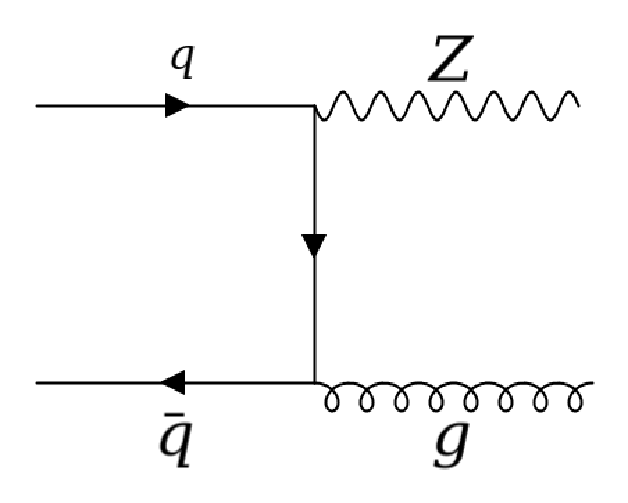
\includegraphics[width=0.4\linewidth]{theory chapter/feynman_z+jet.pdf}
    \caption{A Feynman diagram for the NLO $Z$+jets production process.}
    \label{fig:feynman}
\end{figure}

\subsubsection{$Z$+jets measurement}
\todo{Volevo considerare una misura recente di Z+light jet in ATLAS. Ce n'è un'altra piu' recente a 8 TeV ma ho optato per questa.}

$Z$+jets production has been studied at the ATLAS Experiment in $\sqrt{s} = 13$~TeV collisions with 3.16~fb$^-1$ of data collected during Run 2 in 2015~\cite{ATLAS:2017sag}. The measurement focuses on final states with up to 7 jets of radius $R = 0.4$. Jets are required to have transverse momentum $p_t > 30$~GeV and to be found in the central region. The differential cross section is measured with respect to several different kinematic observables, such as the transverse momentum and rapidity.

Results are compared to predictions obtained with a various MC generators, including LO predictions from \code{MG5\_aMC@NLO}~\cite{Alwall:2014hca} with CKKWL merging with a \code{Pythia8}~\cite{Sjostrand:2007gs} (\code{MG5\_aMC+PY8 CKKWL})parton shower, \code{MG5\_aMC@NLO} with FxFx merging with a \code{Pythia8} shower (MG5\_aMC+PY8 FxFx), and \code{ALPGEN}~\cite{Mangano:2002ea} with a \code{Pythia6}~\cite{Sjostrand:2006za} parton shower (\code{ALPGEN+PY6}), and NLO predictions from \code{Sherpa 2.2.1}~\cite{Gleisberg:2008ta}(\code{Sherpa 2.2}) and NLO fixed order prediction obtained with \code{BLACKHAT}~\cite{Berger:2010vm} generator and showered with Sherpa.

Up to 4 jets can be included in the ME calculation; afterwards, it is necessary to predict the production cross section perturbatively from the parton shower. Predictions are in agreement with data up to $N_\text{jets} = 4$. Afterwards, results diverge. Results and predictions for the cross section are shown in Figure~\ref{fig:z+njets}

\begin{figure}
    \centering
    \includegraphics[width=0.7\linewidth]{theory chapter/z+njets.pdf}
    \caption{The $Z+$jets production cross section as a function of $N_\text{jets}$ compared to predictions obtained with \code{MG5\_aMC+PY8 CKKWL}, \code{MG5\_aMC+PY8 FxFx}, \code{ALPGEN+PY6}, \code{Sherpa 2.2}, and \code{BLACKHAT+Sherpa}~\cite{ATLAS:2017sag}.}
    \label{fig:z+njets}
\end{figure}

\subsubsection{$Z+b$-jets}
For $Z$+jets production with heavy flavours, considerations such as the \emph{flavour scheme} (FS) start to become relevant. The flavour scheme indicates which quarks are found within the proton, i.e.\ whether a given flavour is to be considered as part of the PDF evolution and or if it can only be produced perturbatively. Specifically, a 5FS considers a massless $b$-quark PDF calculated from the evolution of the gluon PDF above the $b$ mass threshold. The massless approximation is valid if $Q^2 \gg m_b^2$. As a $b$-quark PDF is calculate, Feynman diagrams for partonic cross sections with $b$-quarks in the initial state are accessible.
A 4FS, on the other hand, only considers the perturbative production of $b$-quarks in the final state from hard gluon splittings. $b$-quarks are treated as massive, so they are not considered within the proton.  The only contribution thus comes from the ME, though additional contributions from soft gluon splittings in the parton shower are possible in both cases. 
ATLAS has recently published a measurement focusing on final states with $Z+b$-jets and $Z+bb$-jets~\cite{ATLAS:2024tnr}. The measurement is carried out on Run 2 data, corresponding to 139 fb$^{-1}$ and a centre-of-mass energy $\sqrt{s} =13$~TeV. Differential cross sections as a function of variables such as $p_t$ of the $Z$ boson, $p_t$ of the leading $b$-jet, and di-$b$-jet mass $m_{jj}$, and the angular separation between $b$-jets $\Delta\phi_{bb}$ are obtained. Results are compared to a number of NLO predictions, such as \code{MG5\_aMC+PY8} with FxFx merging with both the 4FS and 5FS, Sherpa 2.2, as well as to fixed-order predictions obtained at NLO and NNLO. These are corrected for soft gluon splittings, as will be described in Chapter~\ref{ch:flavLabel}.

Figure~\ref{fig:z+b} shows the cross section as a function of the leading $b$-jet $p_{t,b}$ and $\Delta\phi_{bb}$. For $p_{t,b}$, predictions for the 5FS agree with data better than predictions obtained with the 4FS. Both the NLO and NNLO fixed-order predictions model the data well. For $\Delta\phi_{bb}$, all predictions agree with data within uncertainties, though the 4FS predictions tend to underestimate the data for collinear and back-to-back jets.

\begin{figure}
    \centering
    \includegraphics[width=0.49\linewidth]{theory chapter/ptb.pdf}
    \includegraphics[width=0.49\linewidth]{theory chapter/deltaPhiBB.pdf}
    \caption{The differential cross section for the leading $b$-jet $p_t$ (left) and for the angular separation between di-$b$-jets (right) compared to predictions~\cite{ATLAS:2024tnr}}.
    \label{fig:z+b}
\end{figure}

\subsubsection{$Z+bb$ boosted}

At very high transverse momenta, or boosted regimes, it is possible to execute tests of the Standard Model in extreme phase space. For the $Z+bb$ process in particular, the boosted regime allows us to probe hard and collinear physics.

An ATLAS Run 2 measurement looked at precisely this final state in the boosted regime, mimicking as much as possible the selections for similar boosted Higgs analyses in order to precisely characterise this principal background, composed mainly of gluon splittings. The measurement used $36.1 \text{ fb}^{-1}$ of data collected at $\sqrt{s} = 13$~TeV~\cite{ATLAS:2022uav}.

The measurement studies large-R jets of radius $R = 1.0$ in the central region with a $p_t > 200$~GeV. Jets are tagged through the use of small-R jets of radius $R = 0.2$ with $p_t > 10$~GeV, defined with only track constituents. The $R = 0.2$ jets are identified as $b$-jets by the flavour tagging algorithm \code{MV2c10}~\cite{ATLAS:2018wis} and, if two such jets are associated to a large-R jet using the ghost association criterion\footnote{Cfr.\ Section~\ref{sec:ghost} for a detailed explanation of ghost association.}, then the large-R jet is considered a $b$-jet. Subclasses of flavour are determined by the number of associated small-R jets.

Results are compared to prediction obtained with NLO predictions obtained with Sherpa 2.2.1 with the 5FS, as well as Sherpa 2.2.10 with the 5FS and 4FS variations, and with fusing, which mixes elements of both. Predictions with \code{MadGraph5\_aMC@NLO+Pythia8} were also obtained with 4FS and 5FS variations.

Results for the differential cross section as a function of the large-R jet $p_t$, mass, and angular separation $\Delta R(b,b)$ of the small-R $b$-jets is shown in Figure~\ref{fig:z+bb boosted}. The Sherpa 2.2.10 and \code{MadGraph5\_aMC@NLO} predictions in the 5FS describe the data well. The 4FS Sherpa 2.2.10 and 5FS \code{Sherpa 2.2.10} predictions underestimate the total cross section, while the \code{Sherpa 2.2.10} fusing prediction is close to the \code{Sherpa 2.2.10} 5FS estimate.

\begin{figure}
    \centering
    \includegraphics[width=0.49\linewidth]{theory chapter/z+bjet_boost_pt.pdf}
    \includegraphics[width=0.49\linewidth]{theory chapter/z+b-jet_boost_mass.pdf}\\
    \includegraphics[width=0.49\linewidth]{theory chapter/z+bjet_boost_deltaR.pdf}
    \caption{The differential cross sections as a function of large-R jet $p_t$, jet mass, and angular separation of the small-R $b$-jets for $Z$+bb events~\cite{ATLAS:2022uav}.}
    \label{fig:z+bb boosted}
\end{figure}


\subsection{The Lund Jet Plane}

Since its inception in 2016, a number of measurements of the Lund Jet Plane and related observables have been carried out. The Lund Plane has been measured on inclusive jets by the ATLAS, CMS and ALICE collaborations~\cite{ATLAS:2020bbn, CMS:2023lpp, ALICE:2021yet}. The ATLAS and CMS measurements focus on high-$p_t$ jets, whereas the ALICE measurement looks at jets in a lower $p_t$ range. In Section~\ref{sec:inclusive ljp} we describe in detail the ATLAS and ALICE measurements. We then move on to discussing a measurement of the Lund Jet Plane in heavy flavour jets\cite{LHCb:2025mcq}, and observations of the dead cone effect(\cite{ALICE:2021aqk, CMS:2024gds}). 
For the sake of completeness, we wish to mention a recent ATLAS measurement of the Lund Jet Plane on top and $W$ jets\cite{ATLAS:2024dua}.

\subsubsection{ATLAS measurement on inclusive jets}
\label{sec:inclusive ljp}
The Lund Jet Plane was measured for the first time by the ATLAS collaboration using dijet events from proton-proton collisions at $\sqrt{s}=13$~TeV~\cite{ATLAS:2020bbn}. The measurement uses all data from Run 2, corresponding to 139~fb$^{-1}$.

The measurement focuses on final state with balanced dijet events, of radius $R=0.4$ in the central region. The leading jet is required to have a $p_t^\text{leading} > 675$~GeV, while the subleading jet is required to have a transverse momentum no less than 1.5$\times$ that of the leading jet $p_t^\text{subleading} > p_t^\text{leading}/1.5$. This facilitates the interpretation of the event as a $2\rightarrow 2$ scattering process within QCD.

The Lund Plane is measured exclusively on the \emph{charged} component of the jet. This is required by the higher resolution provided by the tracking system at ATLAS compare to the calorimeter. For more details see Chapter~\ref{ch:atlas}. Tracks are required to have a $p_t > 500$~MeV and to lie in the central region. Tracks are associated to jets by a geometric matching criterion based on the distance in the pseudorapidity-azimuthal angle plane $(\eta, \phi)$\footnote{For a definition of these quantities, see Section~\ref{sec:coordinates}.}. Specifically, the distance $\Delta R(\text{track, jet}) < 0.4$, where the cut-off corresponds to the jet radius. Tracks are clustered into jets using the C/A algorithm. The Lund Jet Plane is then measured on the jets clustered with track constituents. The unfolded particle-level Lund Jet Plane is shown in Figure~\ref{fig:atlas-ljp-inc}.

\begin{figure}
    \centering
    \includegraphics[width=0.7\linewidth]{theory chapter/ljp_atlas_inc.pdf}
    \caption{The particle-level Lund Jet Plane for the charged component of a jet, normalised to the number of jets which pass the event selection~\cite{ATLAS:2020bbn}.}
    \label{fig:atlas-ljp-inc}
\end{figure}

Results are compared to predictions obtained with MC generators including: LO predictions obtained with \code{Pythia v8.230}, NLO predictions obtained with \code{PowHeg}~\cite{Nason:2004rx, Frixione:2007vw, Alioli:2010xa} and showered with \code{Pythia 8.230} (\code{PowHeg+Pythia}), NLO predictions obtained \code{Sherpa 2.2.5} with either the \code{AHADIC}~\cite{Webber:1983if, Winter:2003tt}, a cluster hadronisation model, or the Lund string hadronisation model, and NLO predictions obtained with \code{Herwig 7.1.3}~\cite{Bellm:2017bvx} with either the angle-ordered or dipole parton shower. Figure~\ref{fig:ljp_gen_predictions} shows ratios of the Lund Plane as predicted by these different generators, specifically by varying the LO/NLO ME in \code{Pythia} vs.\ \code{PowHeg+Pythia}, the \code{Herwig} angle-ordered and dipole showers, and the \code{AHADIC} and Lund string hadronisation models in Sherpa. Clear differences arise in the latter two cases, particularly in the regions dominated by hard radiation in the case of the parton shower variation, and in the collinear region in the case of the hadronisation model variation.

\begin{figure}
    \centering
    \includegraphics[width=0.495\linewidth]{theory chapter/ljp_lo_vs_nlo.pdf}
    \includegraphics[width=0.495\linewidth]{theory chapter/ljp_angle_dipole.pdf}\\
    \includegraphics[width=0.495\linewidth]{theory chapter/ljp_ahadic_string.pdf}
    \caption{The ratio of the Lund Jet Planes in dijet events obtained by either varying the order in perturbation theory at which events were generated (top left), the parton shower model (top right), or the hadronisation model (bottom)~\cite{ATLAS:2020bbn}.}
    \label{fig:ljp_gen_predictions}
\end{figure}

The comparison to data was carried out by slicing the Lund Jet Plane and focusing on specific intervals, corresponding to fixing an interval in $\Delta R$ and varying $z$ or vice versa. Figure~\ref{fig:ljp_slices} shows two such slices, by varying $z$ in the region between $0.67 < \log(R/\Delta R) < 1.00$ or by varying $\Delta R$ in the region between $1.80 < \log(1/z) < 2.08$. No single prediction is able to fully describe the data.

\begin{figure}
    \centering
    \includegraphics[width=0.495\linewidth]{theory chapter/ljp_drSlice.pdf}
    \includegraphics[width=0.495\linewidth]{theory chapter/ljp_zSlice.pdf}
    \caption{The results of the dijet measurement of the Lund Jet Plane on inclusive jets compared to various predictions~\cite{ATLAS:2020bbn}.}
    \label{fig:ljp_slices}
\end{figure}

Similar selections are also used to measure the Lund subjet multiplicity, corresponding to the number of emissions in the Lund Plane. Specifically, the number of emissions in just the primary Lund Plane were counted $N^\text{Primary}_\text{Lund}$, as well as the total number of emissions within all Lund Planes $N_\text{Lund}$. The main difference compared to the measurement described above is a decrease in the $p_t$ threshold, down to $p_t > 120$~GeV for both jets. We limit ourselves to citing this result~\cite{ATLAS:2024wrd}.

\subsubsection{ALICE measurement on inclusive jets}
\todo{Forse parlare di questa misura è superfluo? Le piu' importanti sono decisamente ATLAS (in quanto abbiamo ereditato molto da quell'analisi) + LHCb (in quanto unica misura sul LJP su Z+jets)}

ALICE has also looked at the Lund Jet Plane in inclusive jets, but in a much lower $p_t$ range than the ATLAS measurement described above. The measurement focuses on charged particle jets of radius $R= 0.4$ in the $p_t$ range 20-120~GeV produced in the central region in minimum bias events from proton-proton collisions at $\sqrt{s}=13$~TeV. The data corresponds to an integrated luminosity of 22.55 nb$^{-1}$~\cite{ALICE:2021yet}. 

Results are compared to simulations carried out with \code{Pythia8} with the Monash~\cite{Skands:2014pea} tune, \code{Herwig7}, and \code{Sherpa 2.2.8} with the Lund string and \code{AHADIC} hadronisation models. Figure~\ref{fig:alice-ljp} shows the results and the predictions for the projections of the Lund Plane onto the $\ln(R/\Delta R)$ and $\ln(k_t)$ axes in the perturbative region of the plane and for collinear splittings, respectively. For narrow splittings, it is found that the generators disagree at high-$k_t$ by up to 50\%. Agreement is generally within 20\%, though no single prediction fully agrees with the data.

\begin{figure}
    \centering
    \includegraphics[width=0.495\linewidth]{theory chapter/lnRDist_2to5_7to12_March22.png}
    \includegraphics[width=0.495\linewidth]{theory chapter/lnktDist_2to5_5to7_March22.png}
    \caption{The Lund Jet Plane projected onto the $\log(R/\Delta R)$ in a perturbative region ($k_t > 1.0$~GeV) (left) and onto the $\log(k_t)$ axis in a region of collinear splittings ($0.1 < \Delta R < 0.12$)(right)~\cite{ALICE:2021yet}.}
    \label{fig:alice-ljp}
\end{figure}

\subsubsection{LHCb measurement of the light-jet and $b$-jet Lund Plane and their ratio}
\label{sec:ljp_lhcb}
The LHCb Collaboration has recently published a measurement of the Lund Plane in light-quark enriched and $b$-initiated jets~\cite{LHCb:2025mcq}. The data was collected at $\sqrt{13}$~TeV and corresponds to 5.4~fb$^{-1}$ of integrated luminosity. The light-quark enriched sample corresponds to a selection of $Z$+jets events\footnote{The inclusive multijet analyses described above also contain gluon-initiated jets. These are suppressed when considering $Z$+jets.}, while the $b$-initiated sample contains jets containing a fully reconstructed $B^\pm$ meson. This is achieved by reconstructing the $B^\pm \rightarrow J/\psi(\rightarrow \mu^+\mu^-)\pi^\pm$ decay channel.

As LHCb is a forward detector, the measurement exclusively considers jets of radius $R = 0.5$ produced in the forward region, between a rapidity range of $2.5 < y < 4.0$. Jets are also required to have a $p_t > 20$~GeV. A number of jet identification requirements are used to suppress noise and misidentified leptons. The Lund Jet Plane is measured on jets reconstructed with both charged and neutral objects. When constructing the Lund Jet Plane for $B^\pm$ jets, the C/A is undertaken with the WTA recombination scheme, to ensure that the hadron is found within the hardest branch of the jet.

Results are compared to a sample simulated in \code{Pythia8} with the LHCb tune~\cite{LHCb:2010qmd}. In the results, shown in Figure~\ref{fig:lhcb-ljp}, the ratio of the projection onto the $\log(R/\Delta R)$ axis of the Lund Plane for $b$/light jets is also shown. This ratio, as a function of the angular distance $\Delta R$, is sufficient to evince the dead cone effect. At smaller and smaller angles, the $b$-jet Lund Plane is expected to hollow out due to the effect. No such depletion of emissions is expected for light jets. The dead cone effect is thus visible as a decrease in the ratio, at high values of $R/\Delta R$. The comparison of simulation to data also reveals some mismodelling, especially for collinear splittings in $B^\pm$ jets.

\begin{figure}
    \centering
    \includegraphics[width=0.7\linewidth]{theory chapter/ljp_lchb.pdf}
    \caption{The projection onto the $\log(R/\Delta R)$ Lund Plane for light-quark enriched jets and $B^\pm$ jets for forward jets and their ratio, along with a comparison to predictions obtained with Pythia8~\cite{LHCb:2025mcq}.}
    \label{fig:lhcb-ljp}
\end{figure}

%CMS large-R
%CMS dead cone

\subsection{Dead cone effect in CMS}
The LHCb measurement of $B^\pm$-jets is not the first measurement to see the dead cone effect. That honour goes to an ALICE measurement from 2022. This result focused instead on $c$-jets, and fully reconstructed the $D^0$ meson to identify $c$-jets~\cite{ALICE:2021aqk}.

CMS (and ATLAS) do not have the particle-identification capabilities of ALICE and LHCb. As a result, they are generally not capable of fully reconstructing particle decay chains. We will now describe another $b$-jet dead cone measurement, carried out by the CMS Collaboration, which uses flavour tagging techniques reliant on the identification of features typical of heavy flavour jets. These will be described in detail for ATLAS in Section~\ref{sec:ftag}.

The CMS result focuses on the observation of the dead cone effect emerging from the ratio of $b$/inclusive jets and the measurement of substructure observables such as the \code{SoftDrop} groomed jet radius $R_g$, groomed momentum fraction $z_g$ and jet fragmentation function $z_{b,ch}$~\cite{CMS:2024gds}. The measurement was carried out on $301$~pb$^{-1}$ of data from the Run 2 low-pileup proton-proton run at $\sqrt{s} = 5.02$~TeV. Jets of radius $R=0.4$ in the central were identified in multijet final states in a $p_t$ range between 100-120~GeV. The substructure observables are measured on the charged component of the jets only.

Jets originating form bottom-quarks are identified using ParticleNet~\cite{Qu:2019gqs}. The $b$-hadron in the events is partially reconstructed from their charged decay products. Tracks originating from the $b$-hadron decay are identified through a Boosted Decision Tree. The four-momenta of these tracks are summed to reconstruct the charged portion of the $b$-hadron momentum. The dead cone is then observed in the ratio of the groomed jets, as shown in Figure~\ref{fig:cms_deadCone}.

\begin{figure}
    \centering
    \includegraphics[width=0.7\linewidth]{theory chapter/cms_bjet_deadcone.pdf}
    \caption{The ratio of $b$-jets with charged $b$-hadron momentum reconstruction and of inclusive jets in multijet events~\cite{CMS:2024gds}.}
    \label{fig:cms_deadCone}
\end{figure}

A similar dead cone observation was carried out by the CMS Collaboration, focusing on jets containing $D^0$ hadrons~\cite{CMS-PAS-HIN-24-007}.

\todo{Vale la pena parlare anche della misura su jet inclusivi di CMS? Hanno misurato su large-R jets di R=0.8 e rappresenta l'unica misura del LJP su large-R jets finora.}

\subsection{Measurements of jet angularities}
The other substructure observable featuring in this thesis is the jet angularities. The phenomenology of such observables has been extensively studied at colliders for processes such as $Z$+jets~\cite{Reichelt:2021svh} at the LHC, and they have been measured in proton-proton collisions by the ATLAS, CMS and ALICE collaborations on a variety of energies and final states including dijet, $t\bar{t}$, $D^0$-tagged jets and $Z$+jets~\cite{ATLAS:2019kwg, ATLAS:2023jdw, CMS:2021vsp, ALICE:2021njq, Dhankher:2024rkv}. The ALICE Collaboration has additionally measured the angularities in jets arising from Pb-Pb collisions~\cite{ALICE:2024jtb}.

This thesis describes the first ATLAS measurement of the $b$-jet angularities and of the angularities in quark-enriched jets from $Z$+jets. As a result, we briefly describe the CMS measurement of the angularities on $Z$+jets events~\cite{CMS:2021vsp}.

\subsubsection{Jet angularities from dijet and $Z$+jet events in CMS}

The measurement in question analyses 35.9~fb$^{-1}$ of data from proton-proton collisions at $\sqrt{s}=13$~TeV. The generalised angularities $\lambda^1_{0.5}$, $\lambda^1_{1}$, $\lambda^1_{2}$, $\lambda^0_{0}$, and $\lambda^2_{0}$ are measured on groomed and ungroomed jets of radii $R = 0.4$ and $R=0.8$ in a charged-only configuration and with all constituents as a function of $p_t$. Final states identified as $Z$+jets provide a quark-enriched sample of jets, while dijet events are used to extract sample enriched with gluon-initiated jets. Jets are required to be found in the central region and with $p_t > 30$~GeV. The two leading jets $j_1$ and $j_2$ in dijet events are required to be balanced, satisfying $p_t^{j_1} - p_t^{j_2}/p_t^{j_1} - p_t^{j_2} < 0.3$. The same asymmetry requirement is imposed on $j_1$ and the $Z$ candidate in the $Z$+jets region, along with an isolation criterion for $j_1$. For jets in dijet events with $p_t < 1000$~Gev, the most central (lowest $\vert y \vert$) dijet is used for the gluon-enriched sample. This jet is referred to the central dijet, while the other is referred to as the forward dijet. 

Results are compared to simulations obtained at LO with \code{MadGraph5\_aMC@NLO} v2.2.2 showered with \code{Pythia8}  (\code{MG5+Pythia8}) or with \code{Herwig++}~\cite{Bellm:2013hwb, Bahr:2008pv}. Figure~\ref{fig:CMS-LHA} shows the results for $\lambda^1_1$ in the $Z$+jets and central dijet regions for jets with $p_t$ in the range 120-150~GeV. The agreement to data in noticeably worse in the central dijet region for both sets of predictions. In the $Z$+jets region, the \code{MG5+Pythia8} predictions provide the best description of the data.

\begin{figure}
    \centering
    \includegraphics[width=0.495\linewidth]{theory chapter/lha_cms_zjet.pdf}
    \includegraphics[width=0.495\linewidth]{theory chapter/lha_cms_dijet.pdf}

    \caption{The $\lambda^1_1$ angularity measured for ungroomed jets with all constituents in the $p_t$ range 120-150~GeV in $Z$+jet events (left) and in central dijets (right) by CMS~\cite{CMS:2021vsp}.}
    \label{fig:CMS-LHA}
\end{figure}

\end{document}